\chapter{Binary SciDB file format} \label{binForm}
According to SciDB manual web page \cite{scidbBinForm} each binary file represents 1D array, where there are no empty cells in the array (it is dense), but there can be null values for attributes that are nullable. When creating binary files the rules for SciDB attributes are:
\begin{itemize}
\item Attributes in a binary file appear in the same left-to-right order as the attributes of the corresponding array's schema.
\item A fixed-size attribute of length \textit{n} is represented by \textit{n} bytes (in little-endian order).
\item A variable-size attribute of length \textit{n} is represented by a four-byte unsigned integer of value \textit{n}, followed by the n data bytes of the attribute. String attributes include the terminating NUL character (ASCII 0x00) in both the length count and the data bytes.
\item Whether fixed or variable length, a nullable attribute is preceded by a single byte. If a particular attribute value is null, the prefix byte contains the "missing reason code", a value between 0 and 127 inclusive. If not null, the prefix byte must contain 0xFF (-1).
\item Even if a nullable attribute value is in fact null, the prefix byte is still followed by a representation of the attribute: \textit{n} zero bytes for fixed-length attributes of size \textit{n}, or four zero bytes for variable-length attributes (representing a length count of zero).
\item Binary data does not contain attribute separators or cell separators.
\end{itemize}
Among the other characteristics of this format belong:
\begin{itemize}
\item Each cell of the array is represented in contiguous bytes.
\item There are no end-of-cell delimiters.
\item A fixed-length data type that allows null values will always consume one more byte than the data type requires, regardless of whether the value is null or non-null.
\item A fixed-length data type that disallows null values will always consume exactly as many bytes as that data type requires.
\item A string data type that disallows nulls is always preceded by four bytes indicating the string length.
\item The length of a null string is recorded as zero.
\item Every non-null string value is terminated by the NUL character. Even a zero-length string will include this character.
\item The length of a non-null string value includes the terminating NUL character.
\item If a nullable attribute contains a non-null value, the preceding null byte is -1.
\item If a nullable attribute contains a null value, the preceding null byte will contain the missing reason code, which must be between 0 and 127.
\item The file does not contain index values for the dimension of the array to be populated by the LOAD command. The command reads the file sequentially and creates the cells of the array accordingly.
\end{itemize}

Each cell must contain a data type recognizable by SciDB (e.g. native types, user-defined types). Storage format is assumed to be the x86\_64 little-endian.

\chapter{Usage and Types of MAT}\label{appendixMAT}
Typical usage for this algorithm is at nearest neighbour finding query.
In this task the goal is to locate neighbour of the element, which can be done by following ancestor links until finding nearest common ancestor and then descending to the leaf.
For this task there can be used the Spaghettis algorithm \cite{spaghettis} which has only one parameter and it is the number of pivots used. As because the parameter it is clear that the algorithm is pivot based, mapping metric space to k-dimensional vector space. Its competitive algorithm is AESA (Approximating Eliminating Search Algorithm). The distance function of this algorithm has metric properties. Similarity queries solved can be divided into two categories and these are range queries (retrieve all elements which are within distance r to q) and nearest neighbour queries (retrieve the closest elements to q in U). The algorithm steps are: For each pivot calculate and save the distances to each database element. Sort each array saving the permutation with respect to the preceding array (from array to array only the successful traversals are followed). Given k intervals, define k sets (k is number of pivots). Obtain the index intervals corresponding to each set and follow each point through the pointers to find out if it falls inside all the index intervals. If a point falls inside all the index intervals it is in the intersection.

There is also a modification for nearest neighbour queries by selecting unchecked point do range query and if it returns more than one element repeat with lower range else stop. In this case random selection is not totally ineffective.

There is range of types of MAT algorithm, varying from different measures to data organization.
\paragraph{SPAN}
%\subsubsection{SPAN}
The Spacial Piecewise Approximation by Neighbourhoods is the generalized version of MAT algorithm trying to compute maximal homogeneous disks. It is the same for pictures with two values (white/black) as there it is looking for constant values. But it is expensive to compute.
\paragraph{GrayMat}
This algorithm uses Gray-weighted distance. To use it effectively there is a need to segment the picture into two classes. First class is marked as 0 (e.g. background of the picture without objects) and second class is labelled as non 0 (e.g. objects in the picture, not the background).
\paragraph{GradMat}
In this approach there can be computed a specific score for each point P of a picture based on the gradient magnitudes at all pairs of points that have P as their midpoint. These scores are high for points that lie midway between pairs of anti-parallel edges. They define a weighted "medial axis". 
Advantage of this algorithm lies in its sensitivity to noise and irregularities in region edges.
\paragraph{MMMAT}
This variation of the MAT uses Min Max algorithm and is insensitive to noise. It is based on the fact that the MAT of a set S can be constructed by a process of iterative shrinking and re-expanding which corresponds with local MIN and MAX operations. When this construction is used it can be applied to gray-scale pictures. \cite{MMMAT}
\paragraph{QMAT}
Mentioned method is appropriate for processing pictures containing only binary values. It can be imagined that this picture is like an array of $2^n x 2^n$ pixels, which is going to be repeatedly subdivided into quadrants until blocks which consist of a single value are obtained.
Quadtree skeleton then consists of the set of black blocks in the image satisfying three conditions and its radius. The conditions are:
\begin{itemize}
\item Whole image is spanned by the skeleton
\item Elements of skeleton are the blocks with the largest distance transform values
\item No block in the set of blocks but not in the tree requires more than one element of the tree for its subsumation.
\end{itemize}
Each created tree is unique and also has distance value stored in each black node (in white nodes there is no need to store it as there would be 0 value). Example of this method is in this figure \ref{qmat}.


\begin{figure}
\centering
\begin{subfigure}{\textwidth}
\centering
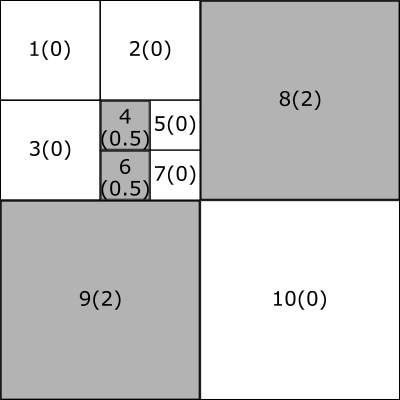
\includegraphics[width=0.5\textwidth]{qmat_picture}
\caption{Sample Image for QMAT processing.}
\end{subfigure}
\vspace{10px}

\begin{subfigure}[t]{.48\textwidth}
 \centering
 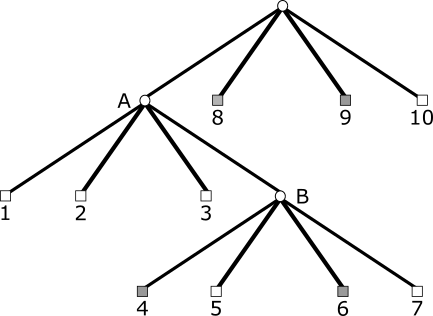
\includegraphics[width=.9\linewidth]{quadtree}
  \caption{Quadtree of the Sample Image.}
\end{subfigure}%
\hfill%
\begin{subfigure}[t]{.48\textwidth}
 \centering
 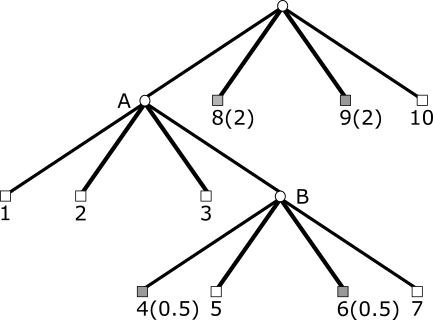
\includegraphics[width=0.9\textwidth]{QMATtree}
 \caption{QMAT tree of the Sample Image.}
\end{subfigure}
\caption{Example of QMAT processing.}
\label{qmat}
\end{figure}


\chapter{ArrayLoop System} \label{arrayLoop}
ArrayLoop is a middle-ware system that translates queries expressed in the model into queries executable by the SciDB. It uses iterative array model, which means there is an array being modified during iteration. Termination condition of this function is represented as an AQL function. This model is interested in major steps that can be decomposed into a minor ones which gives us possibility of parallel evaluation. By major steps its meant that function operates on all cells in array and minor step is otherwise. First of all there is need to assign what to do which is done by \textit{Pi} function. Then it is needed to compute aggregate function separately for each group.  This computation can be done with the help of an algorithm presented in \cite{marginals} and described in the section below \ref{marginals}. After that the records are updated with the new values and this generates new subset containing the results.
For best usage of this algorithm was developed FixPoint function where user specifies the logic of iterative algorithm and it will translate it into ArrayLoop which prepares it into AQL and then SciDB can finally process it.

To transform the function into the AQL format, ArrayLoop first automatically expands and rewrites the operation into an incremental implementation, if it is possible, and efficiently computes the last state of iterative array with the use of the updated cell in each iteration. Then it extracts (for each array chunk) the overlap area of neighbouring chunks and stores this overlaps together with the original chunk which provides both the core and overlap data to the operator during processing. In the final step it identifies outlines of the structures on a low resolution array and then refines details onto high resolution arrays. \cite{arrayloop}

\section{Computing marginals} \label{marginals}
As a marginal of a data cube it can be understood the aggregation of the data in all those tuples that have fixed values in a subset of the dimensions of the cube. Order of the marginal is the number of dimensions over which aggregation is happening. Mapping of reducers q and replication rate r is that no reducer associated with more than q inputs and for every output there is some reducer that is associated with all the inputs that output needs for its computation. Dimensions in this case have same number of different values.
Function $C(n,m,k)$ defines minimum number of sets of size $m$ out of $n$ elements that every set of $k$ out of the same $n$ elements is contained in one of the sets of size $m$, and it is called the covering number.
Different sets of $n,m,k$ are handled differently but when approached with unknown values it can be solved as: one group of handles contains dimensions to $m-k+1$ plus any $k-1$ dimensions from group $2$, and others are formed recursively to cover the dimensions of group $2$ and have none of the members of group $1$.
This problem can be generalized as a problem with weights of dimensions and dividing dimensions into several groups. \cite{marginals}

Example of computing marginal in three dimensional space (as seen in the pictures \ref{margin1} and \ref{margin2}):\\
SELECT SUM(V) \\
FROM DataCube \\
WHERE D1 = x, D2 = y, D3 = z;\\
\begin{figure}
\centering
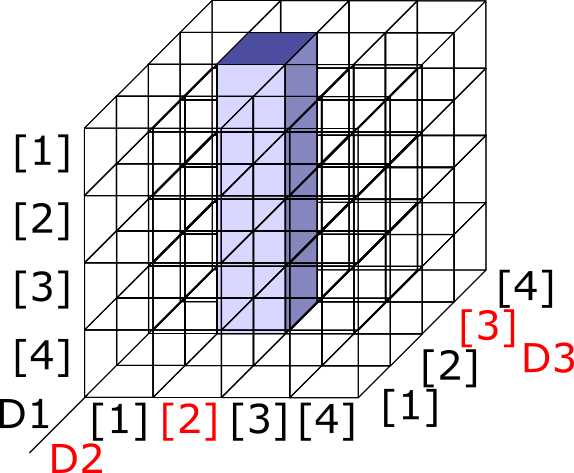
\includegraphics[scale=0.5]{marg1d.png}
\caption{Example of DataCube and selecting dimensions where $y=2$ and $z=3$.}
\label{margin1}
\end{figure}
\begin{figure}
\centering
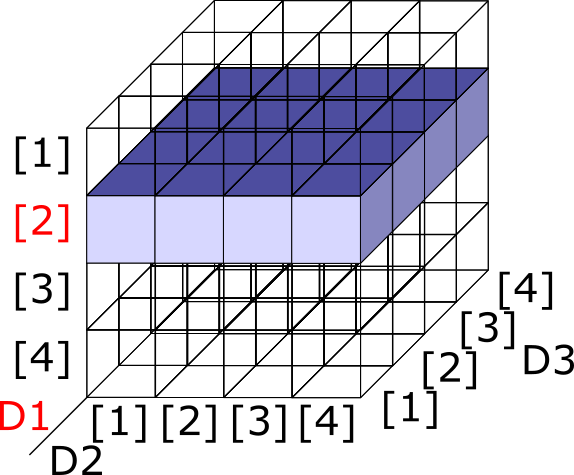
\includegraphics[scale=0.5]{marg2d.png}
\caption{Example of DataCube and selecting dimensions where $x=2$.}
\label{margin2}
\end{figure}

